\documentclass{report}
\usepackage[spanish]{babel}
\usepackage[margin=2cm]{geometry}
\usepackage{graphicx}
\usepackage{float}
\usepackage{titlesec}
\usepackage{caption}
\usepackage{listings}
\usepackage{xcolor}

\definecolor{codegreen}{rgb}{0,0.6,0}
\definecolor{codegray}{rgb}{0.5,0.5,0.5}
\definecolor{codepurple}{rgb}{0.58,0,0.82}
\definecolor{backcolor}{rgb}{0.95,0.95,0.95}


\lstset{
    basicstyle=\ttfamily,
    inputencoding=utf8,
    extendedchars=true,
    literate=%
    {á}{{\'a}}1
    {é}{{\'e}}1
    {í}{{\'i}}1
    {ó}{{\'o}}1
    {ú}{{\'u}}1
    {ñ}{{\~n}}1
    {Á}{{\'A}}1
    {É}{{\'E}}1
    {Í}{{\'I}}1
    {Ó}{{\'O}}1
    {Ú}{{\'U}}1
    {Ñ}{{\~N}}1
}


\lstdefinestyle{mystyle}{
    backgroundcolor=\color{backcolor},
    commentstyle=\color{codegreen},
    keywordstyle=\color{red},
    numberstyle=\tiny\color{codegray},
    stringstyle=\color{codepurple},
    basicstyle=\ttfamily\footnotesize,
    breakatwhitespace=false,
    breaklines=true,
    captionpos=b,
    keepspaces=true,
    numbers=left,
    showspaces=false,
    showstringspaces=false,
    showtabs=false,
    tabsize=2  
}

\titleformat{\section}
{\huge\bfseries}{\thesection.}{1em}{}
\titleformat{\subsection}
{\large\bfseries}{\thesubsection}{1em}{}

\renewcommand\thesection{\arabic{section}}

\title{\Huge{\textbf{Practica 2. Algoritmo genético para codificación de permutaciones.}}\\
\Large{\textbf{Algoritmos Bioinspirados}}}
\author{Diego Castillo Reyes\\Marthon Leobardo Yañez Martinez\\Aldo Escamilla Resendiz}

\graphicspath{{Imagenes/}}

\begin{document}
    \maketitle
    \tableofcontents
    \newpage

    \section{Introducción}
    En esta práctica se implementó un algoritmo genético para resolver el problema de codificación de 
    permutaciones. En especifico encontrar las combinaciones para las soluciones de un cuadrado mágico.
    El cuadrado mágico se refiere a una matriz cuadrada de números enteros en la que la suma de los números 
    en cada fila, columna y diagonal es la misma.\\

    Por ejemplo: 
    %Ejemplo de un cuadrado mágico
    \begin{table}[H]
        \centering
        \begin{tabular}{|c|c|c|}
            \hline
            8 & 1 & 6\\
            \hline
            3 & 5 & 7\\
            \hline
            4 & 9 & 2\\
            \hline
   
        \end{tabular}
        \caption{Ejemplo de un cuadrado mágico}
    \end{table}
    En este ejemplo la suma de los números en cada fila, columna y diagonal es 15.\\
    La idea del algoritmo genético es encontrar la permutación de los números del 
    1 al 9 que formen un cuadrado mágico de tamaño nxn.\\

    \section{Desarrollo}
    Para la implementación del algoritmo genético se utilizó el lenguaje de programación Python.
    %Añade codigo p2.py
    \lstinputlisting[language=Python, style=mystyle]{p2.py}

    \section{Resultados}
    \subsection{Cuadrados mágicos de 3x3}
    En la primera ejecución usando la semilla 1, tardando 6 generaciones, dio como resultado lo siguiente:
    %Agrega la imagen Grafica1.png
    \begin{figure}[H]
        \centering
        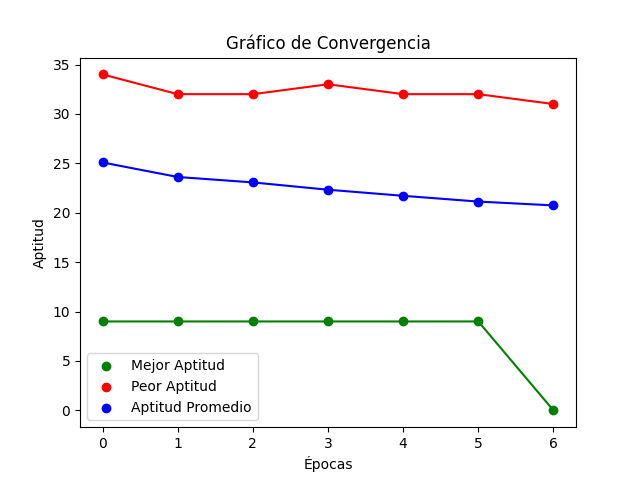
\includegraphics[scale=0.5]{Grafica1.png}
        \caption{Gráfica de la aptitud promedio por generación, Semilla 1}
    \end{figure}
    \begin{table}[H]
        \centering
        \begin{tabular}{|c|c|c|}
            \hline
            2 & 7 & 6\\
            \hline
            9 & 5 & 1\\
            \hline
            4 & 3 & 8\\
            \hline
        \end{tabular}
        \caption{Cuadrado mágico de 3x3, Semilla 1}
    \end{table}
    En la segunda ejecución usando la semilla 3, tardando 37 generaciones, dio como resultado lo siguiente:
    %Agrega la imagen Grafica2.png
    \begin{figure}[H]
        \centering
        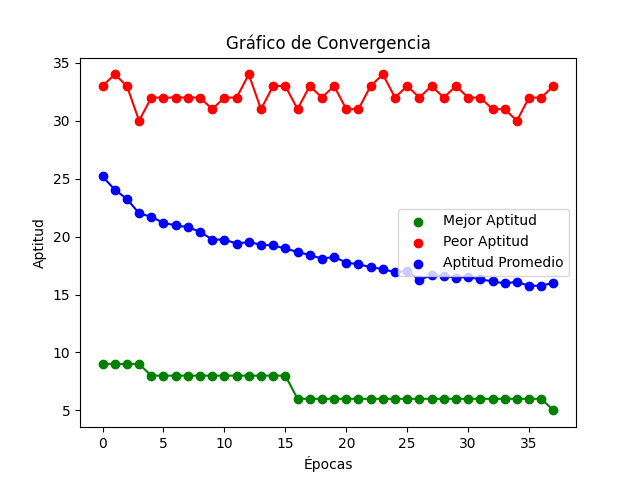
\includegraphics[scale=0.5]{Grafica2.png}
        \caption{Gráfica de la aptitud promedio por generación, Semilla 3}
    \end{figure}
    \begin{table}[H]
        \centering
        \begin{tabular}{|c|c|c|}
            \hline
            8 & 3 & 4\\
            \hline
            2 & 5 & 9\\
            \hline
            6 & 7 & 1\\
            \hline
        \end{tabular}
        \caption{Cuadrado mágico de 3x3, Semilla 3}
    \end{table}
    En la tercera ejecución usando la semilla 5, tardando 73 generaciones, dio como resultado lo siguiente:
    %Agrega la imagen Grafica3.png
    \begin{figure}[H]
        \centering
        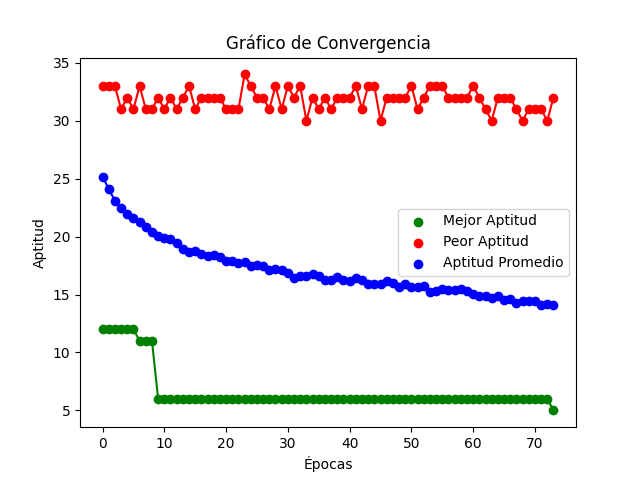
\includegraphics[scale=0.5]{Grafica3.png}
        \caption{Gráfica de la aptitud promedio por generación, Semilla 5}
    \end{figure}
    \begin{table}[H]
        \centering
        \begin{tabular}{|c|c|c|}
            \hline
            4 & 3 & 9\\
            \hline
            8 & 5 & 1\\
            \hline
            2 & 7 & 6\\
            \hline
        \end{tabular}
        \caption{Cuadrado mágico de 3x3, Semilla 5}
    \end{table}
    En la cuarta ejecución usando la semilla 7, tardando 3 generaciones, dio como resultado lo siguiente:
    %Agrega la imagen Grafica4.png
    \begin{figure}[H]
        \centering
        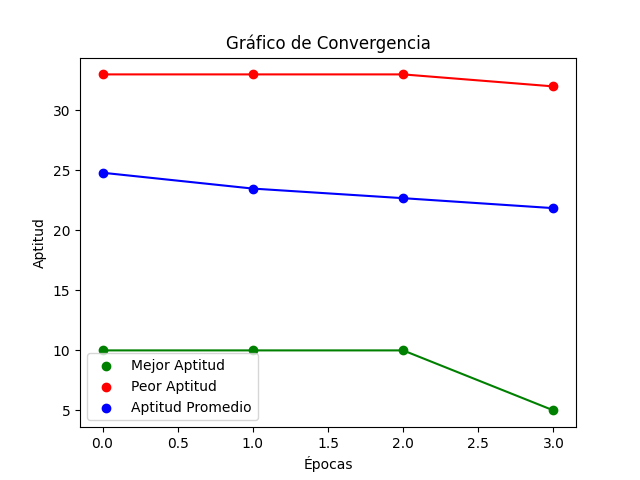
\includegraphics[scale=0.5]{Grafica4.png}
        \caption{Gráfica de la aptitud promedio por generación, Semilla 7}
    \end{figure}
    \begin{table}[H]
        \centering
        \begin{tabular}{|c|c|c|}
            \hline
            6 & 8 & 2\\
            \hline
            1 & 5 & 9\\
            \hline
            7 & 3 & 4\\
            \hline
        \end{tabular}
        \caption{Cuadrado mágico de 3x3, Semilla 7}
    \end{table}
    En la quinta ejecución usando la semilla 11, tardando 21 generaciones, dio como resultado lo siguiente:
    %Agrega la imagen Grafica5.png
    \begin{figure}[H]
        \centering
        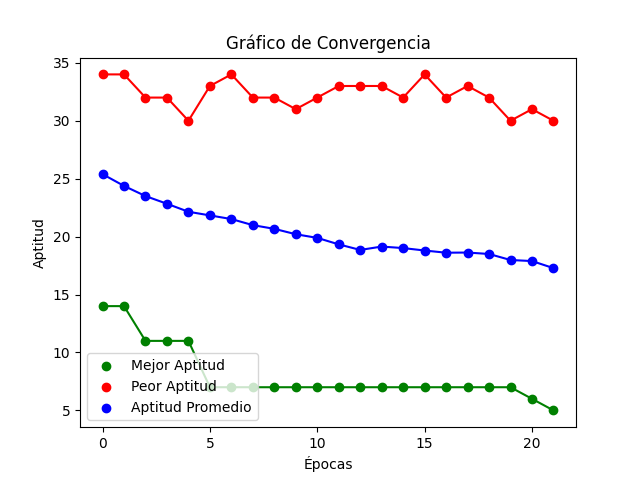
\includegraphics[scale=0.5]{Grafica5.png}
        \caption{Gráfica de la aptitud promedio por generación, Semilla 11}
    \end{figure}
    \begin{table}[H]
        \centering
        \begin{tabular}{|c|c|c|}
            \hline
            4 & 9 & 3\\
            \hline
            2 & 5 & 7\\
            \hline
            8 & 1 & 6\\
            \hline
        \end{tabular}
        \caption{Cuadrado mágico de 3x3, Semilla 11}
    \end{table}
    En la sexta ejecución usando la semilla 13, tardando 23 generaciones, dio como resultado lo siguiente:
    %Agrega la imagen Grafica6.png
    \begin{figure}[H]
        \centering
        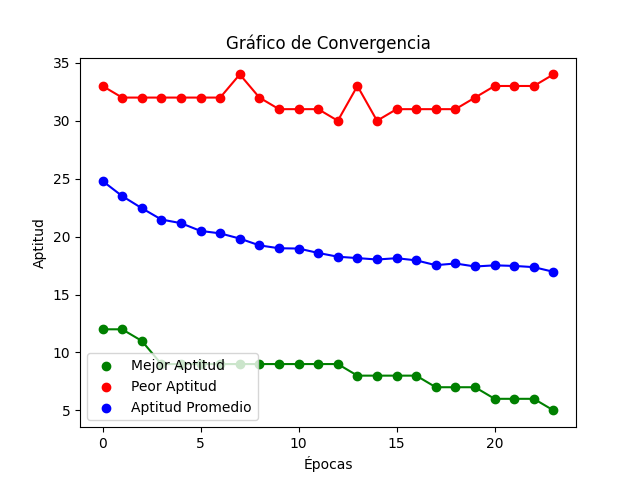
\includegraphics[scale=0.5]{Grafica6.png}
        \caption{Gráfica de la aptitud promedio por generación, Semilla 13}
    \end{figure}
    \begin{table}[H]
        \centering
        \begin{tabular}{|c|c|c|}
            \hline
            4 & 3 & 7\\
            \hline
            9 & 5 & 1\\
            \hline
            2 & 8 & 6\\
            \hline
        \end{tabular}
        \caption{Cuadrado mágico de 3x3, Semilla 13}
    \end{table}
    En la séptima ejecución usando la semilla 19, tardando 48 generaciones, dio como resultado lo siguiente:
    %Agrega la imagen Grafica7.png
    \begin{figure}[H]
        \centering
        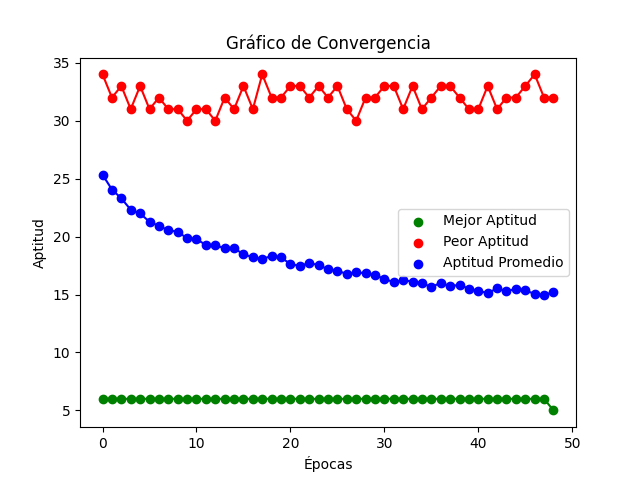
\includegraphics[scale=0.5]{Grafica7.png}
        \caption{Gráfica de la aptitud promedio por generación, Semilla 19}
    \end{figure}
    \begin{table}[H]
        \centering
        \begin{tabular}{|c|c|c|}
            \hline
            8 & 3 & 5\\
            \hline
            1 & 4 & 9\\
            \hline
            6 & 7 & 2\\
            \hline
        \end{tabular}
        \caption{Cuadrado mágico de 3x3, Semilla 19}
    \end{table}
    En la octava ejecución usando la semilla 23, tardando 58 generaciones, dio como resultado lo siguiente:
    %Agrega la imagen Grafica8.png
    \begin{figure}[H]
        \centering
        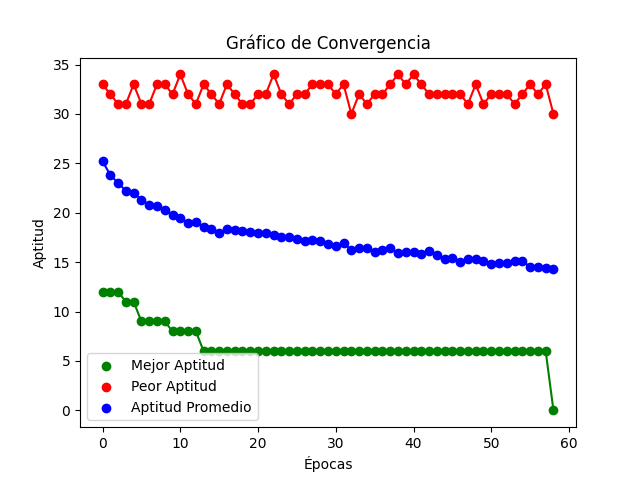
\includegraphics[scale=0.5]{Grafica8.png}
        \caption{Gráfica de la aptitud promedio por generación, Semilla 23}
    \end{figure}
    \begin{table}[H]
        \centering
        \begin{tabular}{|c|c|c|}
            \hline
            4 & 9 & 2\\
            \hline
            3 & 5 & 7\\
            \hline
            8 & 1 & 6\\
            \hline
        \end{tabular}
        \caption{Cuadrado mágico de 3x3, Semilla 23}
    \end{table}

    \subsection{Cuadrados mágicos de 4x4}
    En la primera ejecución usando la semilla 1, tardando 11,002 generaciones, dio como resultado lo siguiente:
    %Agrega la imagen Grafica1_2.png
    \begin{figure}[H]
        \centering
        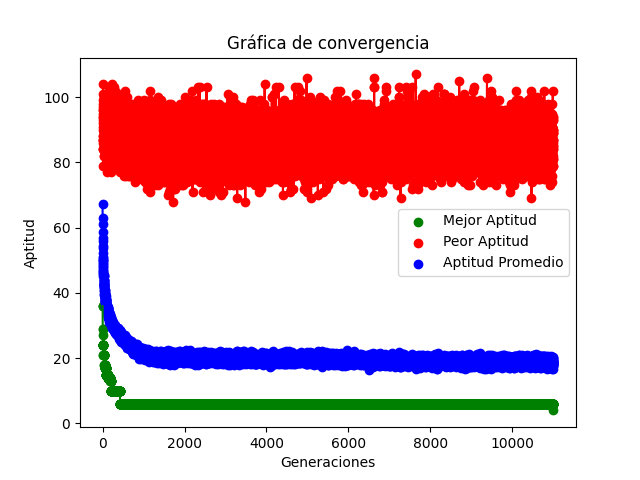
\includegraphics[scale=0.5]{Grafica1_2.png}
        \caption{Gráfica de la aptitud promedio por generación, Semilla 1}
    \end{figure}
    \begin{table}[H]
        \centering
        \begin{tabular}{|c|c|c|c|}
            \hline
            10 & 1 & 14 & 9\\
            \hline
            11 & 4 & 3 & 16\\
            \hline
            5 & 15 & 12 & 2\\
            \hline
            7 & 13 & 6 & 8\\
            \hline
        \end{tabular}
        \caption{Cuadrado mágico de 4x4, Semilla 1}
    \end{table}
    En la segunda ejecución usando la semilla 3, tardando 563 generaciones, dio como resultado lo siguiente:
    %Agrega la imagen Grafica2_2.png
    \begin{figure}[H]
        \centering
        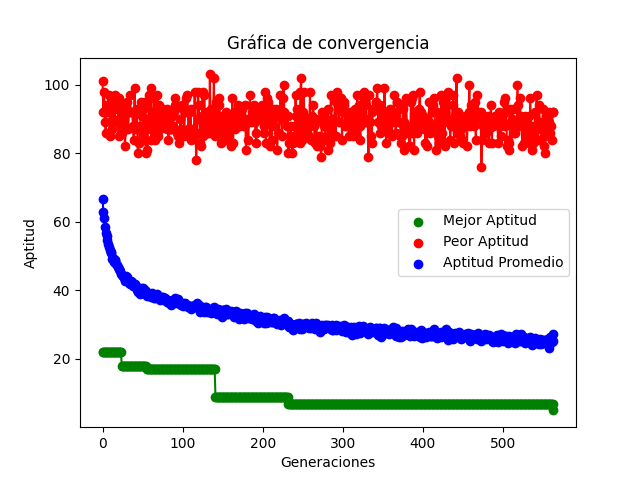
\includegraphics[scale=0.5]{Grafica2_2.png}
        \caption{Gráfica de la aptitud promedio por generación, Semilla 3}
    \end{figure}
    \begin{table}[H]
        \centering
        \begin{tabular}{|c|c|c|c|}
            \hline
            2 & 3 & 15 & 14\\
            \hline
            12 & 16 & 4 & 1\\
            \hline
            9 & 5 & 7 & 13\\
            \hline
            11 & 10 & 8 & 6\\
            \hline
        \end{tabular}
        \caption{Cuadrado mágico de 4x4, Semilla 3}
    \end{table}
    En la tercera ejecución usando la semilla 5, tardando 805 generaciones, dio como resultado lo siguiente:
    %Agrega la imagen Grafica3_2.png
    \begin{figure}[H]
        \centering
        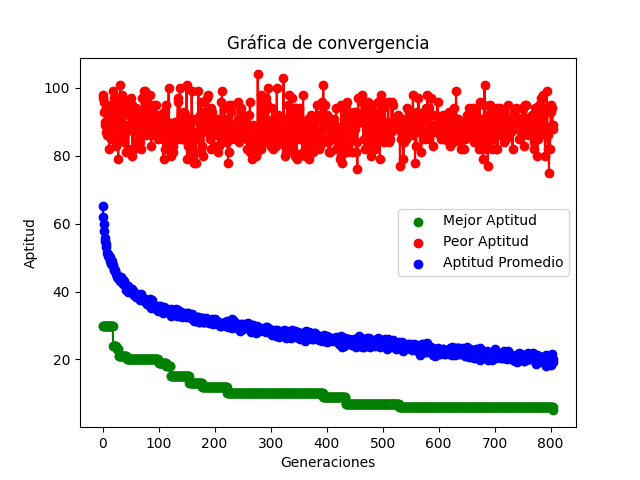
\includegraphics[scale=0.5]{Grafica3_2.png}
        \caption{Gráfica de la aptitud promedio por generación, Semilla 5}
    \end{figure}
    \begin{table}[H]
        \centering
        \begin{tabular}{|c|c|c|c|}
            \hline
            2 & 3 & 15 & 14\\
            \hline
            12 & 16 & 4 & 1\\
            \hline
            9 & 5 & 7 & 13\\
            \hline
            11 & 10 & 8 & 6\\
            \hline
        \end{tabular}
        \caption{Cuadrado mágico de 4x4, Semilla 5}
    \end{table}
    En la cuarta ejecución usando la semilla 7, tardando 823 generaciones, dio como resultado lo siguiente:
    %Agrega la imagen Grafica4_2.png
    \begin{figure}[H]
        \centering
        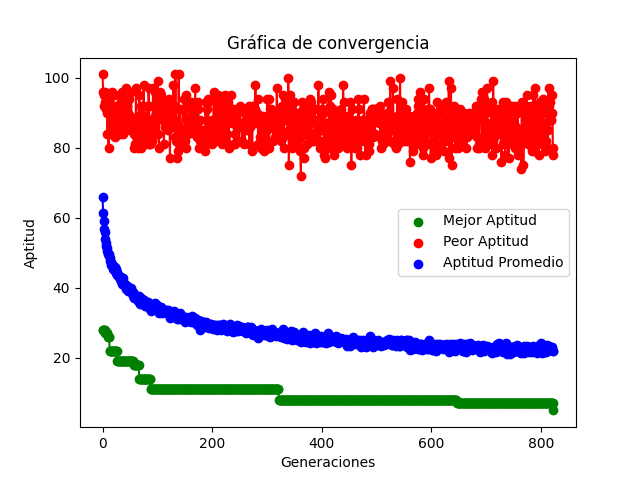
\includegraphics[scale=0.5]{Grafica4_2.png}
        \caption{Gráfica de la aptitud promedio por generación, Semilla 7}
    \end{figure}
    \begin{table}[H]
        \centering
        \begin{tabular}{|c|c|c|c|}
            \hline
            5 & 8 & 10 & 11\\
            \hline
            13 & 4 & 14 & 2\\
            \hline
            12 & 6 & 9 & 7\\
            \hline
            3 & 16 & 1 & 15\\
            \hline
        \end{tabular}
        \caption{Cuadrado mágico de 4x4, Semilla 7}
    \end{table}
    En la quinta ejecución usando la semilla 11, tardando 342 generaciones, dio como resultado lo siguiente:
    %Agrega la imagen Grafica5_2.png
    \begin{figure}[H]
        \centering
        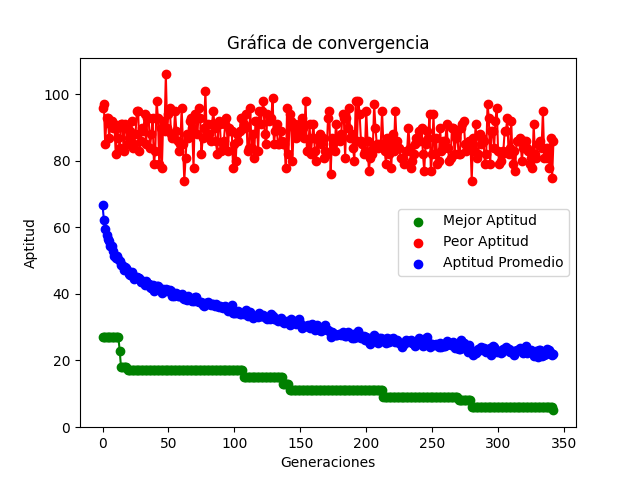
\includegraphics[scale=0.5]{Grafica5_2.png}
        \caption{Gráfica de la aptitud promedio por generación, Semilla 11}
    \end{figure}
    \begin{table}[H]
        \centering
        \begin{tabular}{|c|c|c|c|}
            \hline
            8 & 9 & 4 & 13\\
            \hline
            15 & 14 & 4 & 1\\
            \hline
            16 & 1 & 5 & 12\\
            \hline
            6 & 11 & 10 & 7\\
            \hline
        \end{tabular}
        \caption{Cuadrado mágico de 4x4, Semilla 11}
    \end{table}
    En la sexta ejecución usando la semilla 13, tardando 520 generaciones, dio como resultado lo siguiente:
    %Agrega la imagen Grafica6_2.png
    \begin{figure}[H]
        \centering
        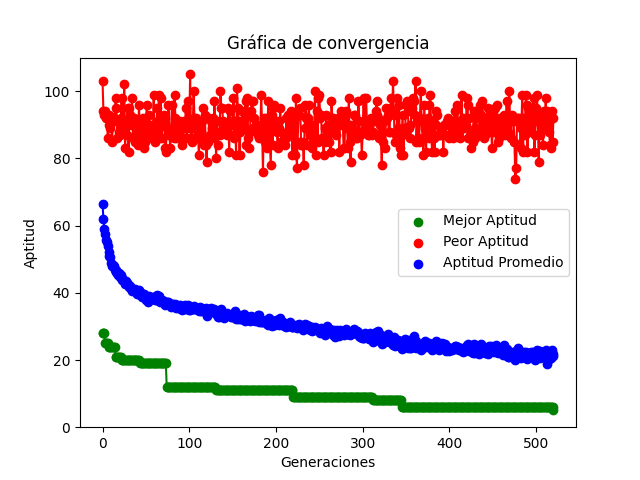
\includegraphics[scale=0.5]{Grafica6_2.png}
        \caption{Gráfica de la aptitud promedio por generación, Semilla 13}
    \end{figure}
    \begin{table}[H]
        \centering
        \begin{tabular}{|c|c|c|c|}
            \hline
            9 & 12 & 5 & 8\\
            \hline
            11 & 7 & 10 & 6\\
            \hline
            2 & 1 & 15 & 16\\
            \hline
            14 & 13& 4 & 3\\
            \hline
        \end{tabular}
        \caption{Cuadrado mágico de 4x4, Semilla 13}
    \end{table}
    En la séptima ejecución usando la semilla 19, tardando 1609 generaciones, dio como resultado lo siguiente:
    %Agrega la imagen Grafica7_2.png
    \begin{figure}[H]
        \centering
        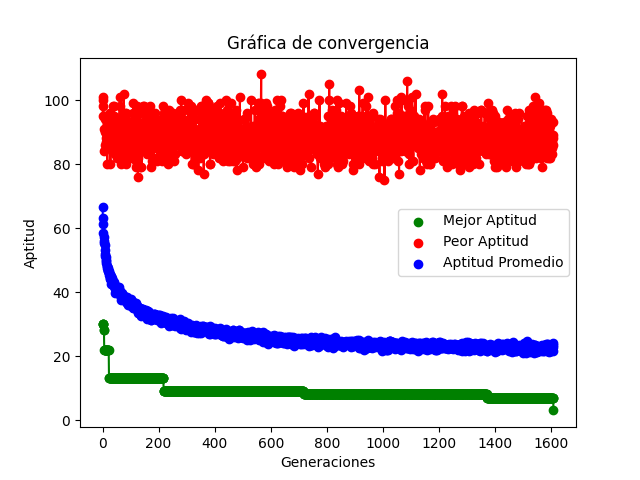
\includegraphics[scale=0.5]{Grafica7_2.png}
        \caption{Gráfica de la aptitud promedio por generación, Semilla 19}
    \end{figure}
    \begin{table}[H]
        \centering
        \begin{tabular}{|c|c|c|c|}
            \hline
            16 & 14 & 1 & 2\\
            \hline
            4 & 3 & 13 & 15\\
            \hline
            5 & 11 & 8 & 10\\
            \hline
            9 & 6 & 12 & 7\\
            \hline
        \end{tabular}
        \caption{Cuadrado mágico de 4x4, Semilla 19}
    \end{table}
    En la octava ejecución usando la semilla 23, tardando 2505 generaciones, dio como resultado lo siguiente:
    %Agrega la imagen Grafica8_2.png
    \begin{figure}[H]
        \centering
        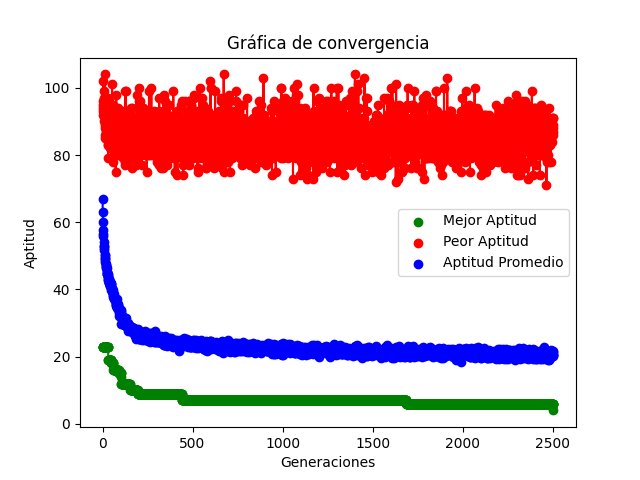
\includegraphics[scale=0.5]{Grafica8_2.png}
        \caption{Gráfica de la aptitud promedio por generación, Semilla 23}
    \end{figure}
    \begin{table}[H]
        \centering
        \begin{tabular}{|c|c|c|c|}
            \hline
            4 & 13 & 9 & 8\\
            \hline
            2 & 14 & 15 & 3\\
            \hline
            16 & 1 & 5 & 12\\
            \hline
            10 & 7 & 6 & 11\\
            \hline
        \end{tabular}
        \caption{Cuadrado mágico de 4x4, Semilla 23}
    \end{table}
    
    \section{Discusión de Resultados}
    •  ¿Cuál fue la función objetivo que encontró más rápido el cuadrado mágico?
    La función que efectivamente puede encontrar más rápido un cuadrado mágico es la parte 
    de la función \textit{verificarexito} que busca una aptitud de 0.0
    Esto se debe a que esta condición identifica directamente un cuadrado mágico perfecto sin errores, y la detección es inmediata 
    tan pronto como se encuentre un individuo con esta aptitud en la población. La evaluación se realiza en cada generación, 
    y tan pronto como se encuentra una aptitud de 0.0, el algoritmo puede terminar, lo que es la manera más rápida de concluir 
    la búsqueda bajo las condiciones ideales.

    La búsqueda de un error mínimo no garantiza un cuadrado perfecto y, además, puede continuar evaluando más individuos incluso después de encontrar cuadrados casi perfectos, lo cual es menos eficiente si el objetivo es encontrar cuadrados mágicos absolutamente precisos.

    •  ¿Cómo modificaría el algoritmo para encontrar todos los posibles cuadrados mágicos? (recuerde que existe más de una solución)
    Diseñar operaciones de cruce que preserven características clave de los cuadrados mágicos, como las sumas de filas, columnas y diagonales. Esto puede ayudar a mantener la viabilidad de las soluciones a través de generaciones.
    Ademar de conservar siempre una copia de los mejores individuos encontrados hasta ahora para asegurarte de que las buenas soluciones no se pierdan a lo largo de las generaciones.

    •  ¿Modificó  los  parámetros  de  su  algoritmo  para  los  diferentes  tamaños  del  cuadrado  mágico(n= 4yn= 5)? Si su respuesta es afirmativa ¿cuáles fueron los parámetros?
    Si, se utilizó parámetros para n = 3 y 4, ya que el tiempo de ejecución con otros parámetros era bastante e incluso llegaba a romperse el programa.\\
    
    Aldo Escamilla: El algoritmo para esta práctica fue diseñado primeramente en inicializar una población, esto quiere decir que, el algoritmo inicia con posibles cuadrados mágicos, donde cada individuo en la población es una permutación aleatoria, después se diseño la funcion de aptitud que para cada cuadrado en la población, se calcula una función de aptitud que mide qué tan cerca está el cuadrado de ser un cuadrado mágico. Esta aptitud se calcula como la suma de las diferencias absolutas entre el número mágico y las sumas de filas, columnas y diagonales del cuadrado, después se hace la elección y la reproducción que la cruce, para después la mutación, con esto, el algoritmo revisa si algún individuo tiene una aptitud de 0.0 o con la otra función se ejecuta hasta que encuentra una solución perfecta.\\

    Leobardo Yañez: En esta practica pude aprender a utilizar algoritmos genéticos para resolver problemas de optimización, en este caso el problema de encontrar cuadrados mágicos. Fue todo un reto ya que tuvimos que implementar funciones para calcular la aptitud de cada individuo, funciones para seleccionar y cruzar a los individuos, y funciones para mutar a los individuos. Fue gratificante al final ya que pude ver como el algoritmo encontraba cuadrados mágicos.\\

    

\end{document}